%! Author = matteomagnini
%! Date = 06/05/26

\documentclass[11pt]{article}

\usepackage{amsmath}
\usepackage{amssymb}
\usepackage{hyperref}
\usepackage{tikz}

\title{
    Intelligent System 2\\
    Tutorial week 12: Structured Argumentation
}

\author{
    Matteo Magnini\\
    \href{mailto:matteo.magnini@uni.lu}{matteo.magnini@uni.lu}
}

\date{
    13 May, 2026
}

\begin{document}

\maketitle

\section{Solutions}

\subsection{Exercise 1}

Facts:
\[
roadLooksWet
\]
\[
mirage
\]

Strict rules:
\[
R_S = \emptyset
\]

Defeasible rules:
\[
r_1: roadLooksWet \Rightarrow roadWet
\]
\[
r_2: roadWet \Rightarrow dangerous
\]
\[
r_3: mirage \Rightarrow \neg roadWet
\]

Therefore:
\[
R_D = \{r_1,r_2,r_3\}
\]

The knowledge base is:
\[
K=(R_S,R_D)
\]

\subsection{Exercise 2}

\textbf{Argument $A_1$}

\[
A_1=[roadLooksWet]
\]

\begin{itemize}
    \item conclusion:
    \[
    cnl(A_1)=roadLooksWet
    \]

    \item subarguments:
    \[
    sub(A_1)=\{A_1\}
    \]

    \item top rule:
    none (ordinary premise)
\end{itemize}

\bigskip

\textbf{Argument $A_2$}

Using:
\[
r_1: roadLooksWet \Rightarrow roadWet
\]

we obtain:
\[
A_2=[A_1]\Rightarrow roadWet
\]

\begin{itemize}
    \item conclusion:
    \[
    cnl(A_2)=roadWet
    \]

    \item subarguments:
    \[
    sub(A_2)=\{A_1,A_2\}
    \]

    \item top rule:
    defeasible
\end{itemize}

\bigskip

\textbf{Argument $A_3$}

Using:
\[
r_3: mirage \Rightarrow \neg roadWet
\]

we obtain:
\[
A_3=[mirage]\Rightarrow \neg roadWet
\]

\begin{itemize}
    \item conclusion:
    \[
    cnl(A_3)=\neg roadWet
    \]

    \item subarguments:
    \[
    sub(A_3)=\{A_3\}
    \]

    \item top rule:
    defeasible
\end{itemize}

\bigskip

\textbf{Argument $A_4$}

Using:
\[
r_2: roadWet \Rightarrow dangerous
\]

and argument $A_2$:
\[
A_4=[A_2]\Rightarrow dangerous
\]

\begin{itemize}
    \item conclusion:
    \[
    cnl(A_4)=dangerous
    \]

    \item subarguments:
    \[
    sub(A_4)=\{A_1,A_2,A_4\}
    \]

    \item top rule:
    defeasible
\end{itemize}

\subsection{Exercise 3}

Recall:
\begin{itemize}
    \item a rebut attack occurs when two arguments conclude opposite literals
    \item attacks propagate to superarguments
\end{itemize}

\bigskip

We have:
\[
cnl(A_2)=roadWet
\]
and
\[
cnl(A_3)=\neg roadWet
\]

Therefore:
\[
A_2 \to A_3
\]
and
\[
A_3 \to A_2
\]

These are rebut attacks.

\bigskip

Now consider propagation.

Since:
\[
A_2 \in sub(A_4)
\]

every attack against $A_2$ propagates to $A_4$.

Hence:
\[
A_3 \to A_4
\]

\bigskip

The abstract argumentation framework is:

\begin{center}
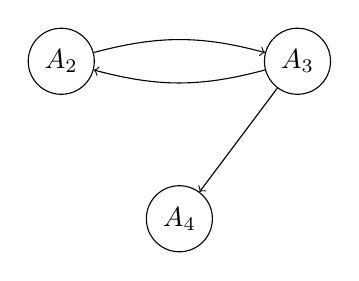
\begin{tikzpicture}
\node[circle,draw] (a2) at (0,0) {$A_2$};
\node[circle,draw] (a3) at (3,0) {$A_3$};
\node[circle,draw] (a4) at (1.5,-2) {$A_4$};

\path[->]
(a2) edge[bend left=15] (a3)
(a3) edge[bend left=15] (a2)
(a3) edge (a4);
\end{tikzpicture}
\end{center}

\bigskip

Is:
\[
\{A_3,A_4\}
\]
conflict-free?

No.

Indeed:
\[
A_3 \to A_4
\]

Therefore the set is not conflict-free.

\subsection{Exercise 4}

We are given:
\[
str(r_1)=1
\]
\[
str(r_2)=3
\]

with:
\[
r_1: roadLooksWet \Rightarrow roadWet
\]
\[
r_2: roadWet \Rightarrow dangerous
\]

Arguments:
\[
A=[roadLooksWet]\Rightarrow roadWet
\]
\[
B=[A]\Rightarrow dangerous
\]

\bigskip

\textbf{Weakest Link}

Under Weakest Link, the strength of an argument is the minimum strength among all defeasible rules used in the argument.

\bigskip

Argument $A$ uses only:
\[
r_1
\]

Therefore:
\[
str_{WL}(A)=1
\]

Argument $B$ uses:
\[
r_1,r_2
\]

Hence:
\[
str_{WL}(B)=\min(1,3)=1
\]

\bigskip

\textbf{Last Link}

Under Last Link, only the last applied defeasible rule matters.

\bigskip

For:
\[
A
\]

the last rule is:
\[
r_1
\]

thus:
\[
str_{LL}(A)=1
\]

For:
\[
B
\]

the last rule is:
\[
r_2
\]

thus:
\[
str_{LL}(B)=3
\]

\bigskip

Therefore:
\begin{itemize}
    \item Weakest Link gives:
    \[
    str(A)=1,\quad str(B)=1
    \]

    \item Last Link gives:
    \[
    str(A)=1,\quad str(B)=3
    \]
\end{itemize}

\bigskip

Last Link gives more importance to the final inference step.

\end{document}
